\section{Inference}
\label{inference}

An important contribution of \affe is its principal type inference.
Our type inference algorithm is
based on the \hmx framework~\citep{DBLP:journals/tapos/OderskySW99},
a Hindley-Milner type system for a language
with constrained types where constraints are expressed in an arbitrary
theory $X$.
%Most importantly,
If $X$ has certain properties, then
\hmx guarantees principal type inference.
We apply \hmx to a concrete constraint language which we name $\CL$.
We adapt and extend \hmx's rules to support kind inference,
track linearity, and handle borrows and regions. We
formulate constraint solving and simplification algorithms for
$\CL$. Finally, we prove that the inference algorithm computes
principal types. 

\subsection{Preliminaries}

In the context of inference, it is critical to know which elements
are input and output of inference judgments.
In the following, when presenting a new judgment,
we write input parameters in \textbf{\textcolor{ForestGreen}{bold
    green}}. The remaining parameters are output parameters.

\paragraph{Usage Environments}

% One novelty of our inference  judgment now
% returns a type environment, which we call ``usage environment'' and commonly
% write $\Sv$, to summarize how variables and borrows are used inside
% the expression.

To determine if a variable is used in an affine manner, we track
its uses and the associated kinds. In the expression
$f\ x\ x$, $x$ is used twice. If $x$ is of type $\tau$, which is of kind $k$,
we add the constraint $\Cleq{k}{\kun}$.
%
To infer such constraints, our inference judgment not only
takes an environment as parameter but also returns a \emph{usage
  environment}, denoted $\Sv$, 
which summarizes usages of variables and borrows.
Usage environments are defined like normal environments.
%
In \cref{sdtyping}, we use relations to split environments and to
transform suspended bindings into borrows inside a region.
These relations take a constraint parameter which validates
the transformations.
In the context of inference, we define new judgments which \emph{infer}
the constraints.
\begin{itemize}[leftmargin=*,topsep=0pt]
\item $\bsplit{C}{\Sv}{\inP{\Sv_1}}{\inP{\Sv_2}}$.
  Given two usage environments $\inP{\Sv_1}$ and $\inP{\Sv_2}$,
  we return $\Sv$, the merged environment, and $C$, a set
  of constraints that must be respected.
\item $\bregion[\inP{n}]{C}{\inP{x}}{\Sv}{\inP{\Sv'}}$.
  Given a usage environment $\inP{\Sv'}$, a nesting level $\inP{n}$,
  and a variable name $\inP{x}$, we return
  $\Sv$ where the borrow binding of $x$ in $\Sv'$, if it exists,
  is replaced by
  a suspended binding. We also return the constraints $C$.
\end{itemize}
Both relations are total and non-ambiguous in term of their input
(i.e., functions), and use
the rules presented in \cref{sdtyping:split,sdtyping:regions}.
%
The relations used for syntax-directed typing can trivially be defined
in terms of these new relations by using constraint entailment.
All relations are fully described in Appendix D.

\paragraph{Constraint Normalization}

The \hmx framework assumes the existence of a function
``$\operatorname{normalize}$'' which takes a constraint $\inP{C}$ and a
substitution $\inP\psi$ and returns a 
simplified constraint $C'$
and an updated substitution $\unif'$.
Normalization returns a normal form such that $\unif'$ is a most general unifier.
For now, we simply
assume the existence of such a function for our constraint system
and defer details to \cref{infer:solving}.

\subsection{Type Inference}

We write $\inferW{\Sv}{(C,\unif)}{\inP{\E}}{\inP{e}}{\tau}$ when
$\inP{e}$\ has type $\tau$ in $\inP{\E}$ under the constraints $C$ and unifier $\unif$
with a usage environment $\Sv$. $\inP\E$ and $\inP{e}$ are the input parameters of our
inference algorithm.
Unlike in the syntax-directed version, $\E$ contains only regular and type bindings.
Suspended and borrow bindings can only be present in $\Sv$.
We revisit some of the syntax-directed rules presented in \cref{sdtyping}
to highlight the novelties
of our inference algorithm and the differences with the syntax-directed
system in \cref{rule:infer:envs}.
The complete type inference rules are shown in Appendix E.

\paragraph{Environments and Bindings}
\label{infer:envs}
%
\begin{figure*}[tb]
  \begin{mathpar}
    \ruleIVar
    \and
    \ruleIAbs
    \and
    % \ruleILet
    % \hfill
    \ruleIRegion
    % \and
    % \ruleIPair
    \and
    \ruleIApp
    \and
    \inferrule{}
    { \Weaken_{\bvar{x}{\sigma}}(\Sv) =
      \text{if } (x\in\Sv) \text{ then} \Ctrue \text{else }
      \Cleq{\sigma}{\kaff_\infty}
      % \begin{dcases}
      %   \Ctrue&\text{if } x\in\Sv\\
      %   \Cleq{\sigma}{\kaff_\infty}&\\
      % \end{dcases}
      % \\\\\\
      % \generalize{C}{\E}{\tau} =
      % (\Cproj{(\Multi{\kvar},\Multi{\tvar})}{C},
      % \forall (\Multi{\kvar},\Multi{\tvar}).\qual{C}{\tau})\\
      % \text{ where}\\\\
      % \Multi{\kvar},\Multi{\tvar} = (\fv{\tau}\cup\fv{C})\setminus\fv{\E}
    }
  \end{mathpar}
  \vspace{-15pt}
  \caption{Selected inference rules -- $\inferW{\Sv}{(C,\unif)}{\inP{\E}}{\inP{e}}{\tau}$}
  \label{rule:infer:envs}
  \label{rule:infer:envrules}
  \label{rule:infer:let}
\end{figure*}
%
In the syntax-directed system, the {\sc Var} rule ensure
that linear variables are not discarded at the \emph{leaves}.
In the inference algorithm, we operate in the opposite
direction: we collect data from the leaves and enforce linearity
at \emph{binders}. This policy is reflected in the {\sc Var$_I$} and
{\sc Abs$_I$} rules.
Typing for variables is very similar to traditional Hindley-Milner
type inference. To keep track of linearity, we record
that $x$ was used with the scheme $\schm$ by returning
a usage environment $\Sv = \{ \bvar{x}{\schm} \}$.
%
This usage environment is in turn used at each binder to enforce proper
usage of linear variable via the $\Weaken$ property as shown for
lambda expressions in the {\sc Abs$_I$} rule.
First, we typecheck the body of the lambda and obtain a usage
environment $\Sv_x$. As in the syntax-directed type system,
we introduce the constraint
$\Cleq{\Sv\Sdel{x}}{\kvar}$ which properly accounts for captures in
the body of the lambda expression. We then introduce the constraint
$\Weaken_{\bvar{x}{\sigma}}(\Sv)$, which fails if we try
to abandon a linear variable. 
The $\Weaken$ constraint is introduced at each binding construct.
%
Finally, we normalize constraints to ensure
that the inference algorithm always return the simplest possible
constraints and unifiers.



\paragraph{Splitting and Regions}
\label{infer:split}
\label{infer:regions}

Inference versions
of the {\sc App} and {\sc Region} rules
are similar to the original ones, but now \emph{return} the usage
environment $\Sv$.
As such, we use the ``inference'' version of the relations on
the environment,
$\bsplit{C}{\Sv}{\inP{\Sv_1}}{\inP{\Sv_2}}$
and $\bregion{C}{\inP{x}}{\Sv}{\inP{\Sv'}}$,
which returns the necessary constraints.
We then collect all constraints and normalize them.

\subsection{Constraints}
\label{infer:solving}



\newcommand\A{\mathcal A}
\newcommand\SC{\mathcal S}



%
% \begin{figure}[tb]
%   \centering
%   \begin{align*}
%     C &::= \Cleq{\tau_1}{\tau_2}
%         \mid \Cleq{k_1}{k_2}
%         \mid C_1 \Cand C_2
%         \mid \Cproj{\tvar}{C}
%         \mid \Cproj{\kvar}{C}
%   \end{align*}
%   \caption{The constraint language}
%   \label{grammar:constraint}
%   % \begin{minipage}{0.65\linewidth}
  \begin{mathpar}
    \inferrule[Lat-UAL]{}{\kun \lk \kaff \lk \klin}
    \and
    \inferrule[Lat-Level]{\mul \lk \mul' \and n \lk n'}{\mul_n \lk_\Lat \mul'_{n'}}
  \end{mathpar}
\end{minipage}~
\begin{minipage}{0.2\linewidth}
  \centering
  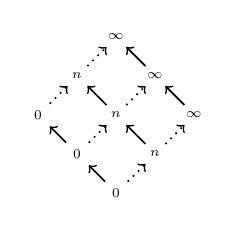
\begin{tikzpicture}
    [->,auto,semithick, every node/.style={scale=0.7}]
    \node(U) {$\kun_0$} ;
    \node(A) [above left of=U] {$\kaff_0$} ;
    \node(L) [above left of=A] {$\klin_0$} ;
    \node(Un) [above right of=U] {$\kun_n$} ;
    \node(An) [above left of=Un] {$\kaff_n$} ;
    \node(Ln) [above left of=An] {$\klin_n$} ;
    \node(Uinf) [above right of=Un] {$\kun_\infty$} ;
    \node(Ainf) [above left of=Uinf] {$\kaff_\infty$} ;
    \node(Linf) [above left of=Ainf] {$\klin_\infty$} ;
    \path
    (U) edge (A)
    (A) edge (L)
    (Un) edge (An)
    (An) edge (Ln)
    (Uinf) edge (Ainf)
    (Ainf) edge (Linf)
    ;
    \path[dotted]
    (U) edge (Un)
    (A) edge (An)
    (L) edge (Ln)
    (Un) edge (Uinf)
    (An) edge (Ainf)
    (Ln) edge (Linf)
    ;
  \end{tikzpicture}
\end{minipage}

%%% Local Variables:
%%% mode: latex
%%% TeX-master: "../main"
%%% End:

%   % \caption{Lattice inequalities -- $k \lk_\Lat k'$}
%   \begin{mathpar}
  \inferrule
  {}{ \entail{}{\Cleq{\kvar}{\kaff}} }
  \and
  \inferrule
  {}{ \entail{}{\Cleq{\kun}{\kvar}} }
  \and
  \inferrule
  {}{ \entail{}{\Cleq{\kvar}{\kvar}} }
  \and
  % \inferrule
  % {\Cleq{k}{k'} \in C}{ \entail{C}{\Cleq{k}{k'}} }
  % \and
  % \inferrule
  % { \entail{C}{\Cleq{x_1}{x}}\\
  %   \entail{C}{\Cleq{x}{x_2}}
  % }
  % { \entail{C}{\Cleq{x_1}{x_2}} }
  % \and
  % \inferrule
  % { \entail{C}{D} }
  % { \entail{C}{\Cproj{x}{D}} }
  % \\
  \inferrule
  { \entail{C}{\Cleq{\tau'_1}{\tau_1}}\\
    \entail{C}{\Cleq{\tau_2}{\tau'_2}}\\
    \entail{C}{\Cleq{k}{k'}}
  }
  { \entail{C}{\Cleq{\tau_1\tarr{k}\tau_2}{\tau'_1\tarr{k'}\tau'_2}} }
  \and
  \inferrule
  { \forall i,\ \entail{C}{\Cleq{\tau_i}{\tau_i}}\\
  }
  { \entail{C}{\Cleq{\tapp{t}{(\tau_i)}}{\tapp{t}{(\tau'_i)}}} }
  \and
  
  % \and
  % \inferrule
  % { \entail{C}{\Cleq{k}{k'}} \\
  %   \entail{C}{\Cleq{k'}{k}} }
  % { \entail{C}{\Ceq{k}{k'}} }
  % \and
  % \inferrule
  % { \entail{C}{\Cleq{k}{k'}} }
  % { \entail{C}{\Ckind{\tau_0\tarr{k}\tau_1}}{k'}}
  % \and
  % \text{Completion to form a cylindric constraint system.}
\end{mathpar}

%%% Local Variables:
%%% mode: latex
%%% TeX-master: "../main"
%%% End:

%   \caption{Base entailment rules -- $\entail{\inP{C}}{\inP{D}}$ }
%   \label{rules:entail}
% \end{figure}

To properly define our type system, we need to define $\CL$, a constraint
system equipped with an entailment relation noted $\operatorname{\vdash_e}$
and a normalizing function.
For concision, we first demonstrate the constraint solving
algorithm with an example. We then state the various properties
that make it suitable for use in the \hmx framework.
The complete constraint system is
defined in Appendix C.

\subsubsection{Constraints Normalization by Example}

\label{solving:example}

\begin{figure}[tbp]
  \centering
  \begin{tikzpicture}[node distance=6mm,xscale=1.2,yscale=0.7,.every edge/.style=[link,->,>=latex,thick]]
    \node (U) {$\kun$} ;
    \node[above left=of U] (x) {$\kvar_x$} ;
    \node[above=of x] (r) {$\kvar_r$};
    \node[left=of x] (g) {$\kvar_\gamma$} ;
    \node[right=of x] (b) {$\kvar_\beta$} ;
    \node[right=of b] (3) {$\kvar_3$} ;
    \node[above=of 3] (f) {$\kvar_f$} ;
    \node[above=of f] (1) {$\kvar_1$} ;

    \draw (x) to[bend right] (U) ;
    \draw (x) -> (r) ;
    \draw (b) -> (r) ;
    \draw (g) -> (x) ;
    \draw (3) -> (f) ;
    \draw (f) -> (1) ;

    \draw[blue] (3) to[bend right] (1);

    \node at (-0.5,-0.5) {Before};
    
    \begin{scope}[dashed,gray]
      \draw (U) to[bend right] (x) ;
      \draw (U) to (b) ;
      \draw (U) to[bend left] (g) ;
      \draw (U) to (r) ;
      \draw (U) to (1) ;
      \draw (U) to (3) ;
      \draw (U) to (f) ;
    \end{scope}
  
    \begin{scope}[on background layer]
      \node[fill=green!20,draw=green,
      inner sep=-1pt,ellipse,rotate fit=-20,fit=(U.south) (x) (g)] {};
      \node[fill=red!20,draw=red, inner sep=-2pt, circle,fit=(r)] {};
      \node[fill=red!20,draw=red, inner sep=-2pt, circle,fit=(f)] {};
    \end{scope}
  \end{tikzpicture}~
  \vrule~
  \begin{tikzpicture}[node distance=7mm,every edge/.style=[link,->,>=latex,thick]]
    \node (b) {$\kvar_\beta$} ;
    \node[right=of b] (3) {$\kvar_3$} ;
    \node[above=of 3] (f) {} ;
    \node[above=of f] (1) {$\kvar_1$} ;

    \draw (3) to[bend right] (1);

    \node at (0.5,-1.5) {After};
  \end{tikzpicture}
  \vspace{-5pt}
    \caption{Graph representing the example constraints}
    \label{example:graph}
    % \caption{Final state of the graph}
    \label{example:graph:final}
\end{figure}

Consider the expression $\lam{f}{\lam{x}{(\app{f}{x},x)}}$.
The inference algorithm yields the following constraints:
%
\begin{align*}
  \E &= (\tvar_f : \kvar_f)
  (\tvar_x : \kvar_x)\dots\\
  C &= (\tvar_f \leq \gamma \tarr{\kvar_1} \beta )
  \Cand
  (\gamma \leq \tvar_x)
  \Cand
  (\beta \times  \tvar_x \leq \alpha_r)
  \Cand
  (\kvar_x \leq \kun)
\end{align*}

The first step of the algorithm uses Herbrand unification to obtain
a type skeleton. 
$$
(\gamma \tarr{\kvar_3} \beta) \tarr{\kvar_2} \gamma \tarr{\kvar_1} \beta \times  \gamma$$

In addition, we obtain the following kind constraints: 
\[\begin{aligned}
    % \Cproj{\kvar_r}\Cproj{\kvar_f}\Cproj{\kvar_x}{}
    &(\kvar_x \leq \kun)
    \Cand
    (\kvar_\gamma \leq \kvar_x)
    \Cand
    (\kvar_x \leq \kvar_r)
    \Cand
    (\kvar_\beta \leq \kvar_r)
    \Cand
    (\kvar_3 \leq \kvar_f)
    \Cand
    (\kvar_f \leq \kvar_1)
\end{aligned}\]
% Since $\kvar_r$, $\kvar_f$ and $\kvar_x$ are not present in the type skeleton,
% they are existentially quantified.

We translate these constraints into a relation whose graph
is shown in \cref{example:graph}.
%
The algorithm then proceeds as follow:
\begin{itemize}[noitemsep]
\item From the constraints above, we deduce the graph shown
  with plain arrows on the left of \cref{example:graph}.
\item We add all the dashed arrows by saturating
  lattice inequalities. For clarity, we only show $\kun$.
\item We identify the connected component circled in
  {\color{ForestGreen} green}.
  We deduce $\kvar_\gamma = \kvar_x = \kun$.
\item We take the transitive closure, which adds the
  arrow in {\color{blue} blue} from $\kvar_3$ to $\kvar_1$.
\item We remove the remaining nodes not present in the type skeleton (colored in {\color{red} red}): $\kvar_r$ and $\kvar_f$.
\item We clean up the graph (transitive reduction, remove unneeded constants, \dots),
  and obtain the graph shown on the right.
  We deduce $\kvar_3 \leq \kvar_1$.
\end{itemize}

The final constraint is thus
$$\kvar_\gamma = \kvar_x = \kun \Cand \kvar_3 \leq \kvar_1$$
If we were to generalize, we would obtain the type scheme:
$$\forall \kvar_\beta \kvar_1 \kvar_2 \kvar_3
(\gamma : \kun) (\beta : \kvar_\beta).\ %
\qual
{\Cleq{\kvar_3}{\kvar_1}}
{(\gamma \tarr{\kvar_3} \beta) \tarr{\kvar_2} \gamma \tarr{\kvar_1} \beta \times  \gamma}$$

We can further simplify this type by exploiting variance. As $\kvar_1$
and $\kvar_2$ are only used in covariant position, they can be
replaced by their lower bounds, $\kvar_3$ and $\kun$. 
By removing the unused quantifiers, we obtain a much simplified equivalent type:
$$
\forall \kvar
(\gamma : \kun).
{(\gamma \tarr{\kvar} \beta) \tarr{} \gamma \tarr{\kvar} \beta \times  \gamma}$$



%%% Local Variables:
%%% mode: latex
%%% TeX-master: "../main"
%%% End:



\subsubsection{Properties of the Constraint System}

To apply \hmx to $\CL$, normalize must compute principal normal forms
and $\CL$ must be regular.

\begin{property}[Principal normal form]
  Normalization computes principal normal forms for $\CL$, i.e.
  given a constraint $D\in\CL$, a substitution $\phi$ and
  $(C,\unif) = \normalize{D}{\phi}$,
  then $\phi\leq\unif$,
  $C \equivC \unif D$ and
  $\unif C = C$.
\end{property}

\begin{property}[Regular constraint system]
  $\CL$ is regular, ie, for $x, x'$ two types or kinds,
  $\entail{}{\Ceq{x}{x'}}$ implies
  $\fv{x} = \fv{x'}$
\end{property}

These properties
are sufficient to state that $HM(\CL)$ provides principal type inference.
The next section shows that these properties carry over to the
inference algorithm for our extension
of \hmx
with kind inference, affine types, and borrows.
%
This algorithm includes sound and complete constraint simplification.
In addition, we may add ``best-effort'' simplification
rules which help reduce the size of inferred signatures 
\citep{DBLP:conf/aplas/Simonet03}.

\subsection{Soundness and Principality}

The extended inference algorithm is sound
and complete with respect to our extension of \hmx.
% This is achieved by extending
% the original proofs from \hmx, which is done in \cref{appendix:infer}.
%
The first theorem states that inference is sound
with respect to the syntax-directed type system.

\begin{theorem}[Soundness of inference]
  Given a type environment $\E$ containing only value bindings,
  $\E|_\tau$ containing only type bindings, and a term $e$:\\
  if $\inferW{\Sv}{(C,\unif)}{\E;\E_\tau}{e}{\tau}$\\
  then $\inferS{C}{\unif(\Sv;\E_\tau)}{e}{\tau}$, $\unif C = C$ and $\unif \tau = \tau$
\end{theorem}

The syntax-directed derivation holds with the usage environment $\Sv$ instead of the originally provided environment $\E$. Indeed,
$\E$ does not contain suspended and borrow bindings. Those
are discovered on the fly and recorded in $\Sv$. Type bindings
are taken directly from the syntax-directed derivation.

The second theorem states that inference is complete: for any given
syntax-directed typing derivation, our inference algorithm can find
a derivation that gives a type at least as general.
% For this, we need first to provide a few additional definitions.

% \begin{definition}[More general unifier]
%   Given a set of variable $U$ and $\unif$, $\unif'$ and $\phi$
%   substitutions. \\
%   Then
%   $\unif \leq^{\phi}_{U} \unif'$ iff $(\phi \circ \unif)|_{U} = \unif'|_U$.
% \end{definition}

\begin{definition}[Instance relation]
  Given a constraint $C$ and two schemes
  $\schm = \forall \Multi\tvar. \qual{D}{\tau}$ and
  $\schm' = \forall \Multi\tvar'. \qual{D'}{\tau'} $.
  Then $\entail{C}{\schm \preceq \schm'}$
  iff $\entail{C}{\subst{\tvar}{\tau''} D}$
  and $\entail{C\Cand D'}{\Cleq{\subst{\tvar}{\tau''}\tau}{\tau'}}$
\end{definition}

\begin{definition}[Flattened environment]
A flattened environment,
written as $\Eflat\E$, is the environment
where all the binders are replaced by normal ones. More formally:
\begin{align*}
  \Eflat\E
  =& \left\{\bvar{x}{\tau}\in\E \mid
    \vee \bvar{\borrow{x}}{\borrowty{k}{\tau}}\in\E
    \vee \svar{x}{\tau}^n\in\E
    \right\}
     \cup \left\{ \bvar{\tvar}{k} \mid \bvar{\tvar}{k}\in\E \right\}
\end{align*}
\end{definition}


% We can then state principality.

% \begin{theorem}[Completeness]
%   Given $\inferS{C'}{\E'}{e}{\tau'}$ and
%   $\entail{}{\unif'\E \preceq \E'}$.
%   Then $$\inferW{\Sv}{(C,\unif)}{\Eflat\E}{e}{\tau}$$
%   for some environment $\Sv$,
%   substitution $\unif$, constraint $C$ and type $\tau$ such
%   that
%   \begin{align*}
%     \unif &\leq^{\phi}_{\fv{\E}} \unif'
%     &\entail{C'&}{\phi C}
%     &\entail{&}{\phi \schm \preceq \schm'}
%     &\Sv&\subset\E
%     % &( C, \schm, \unif) &\leq (C',\schm',\unif')
%   \end{align*}
%   where $\schm' = \generalize{C'}{\E'}{\tau'}$
%   and $\schm = \generalize{C}{\E}{\tau}$
% \end{theorem}

% Finally, principality is a direct application of completeness to
% toplevel programs.

\begin{theorem}[Principality]
  Let $\inferS{\Ctrue}{\E}{e}{\schm}$ a closed typing judgment.
  Then $\inferW{\Sv}{(C,\unif)}{\Eflat\E}{e}{\tau}$
  such that:
  \begin{align*}
    (\Ctrue,\schm_o) &= \generalize{C}{\unif\E}{\tau}
    &\entail{&}{\schm_o \preceq \schm}
    % &( C, \schm, \unif) &\leq (C',\schm',\unif')
  \end{align*}


\end{theorem}

%%% Local Variables:
%%% mode: latex
%%% TeX-master: "../main"
%%% End:
